%======================================================================
\chapter{From prediction--correction to LATIN and the direct cyclic method}\label{ch:pl-cyc}
%======================================================================
% Sources: notes "Global-local methods for cyclic and monotone elastoplasticity"
% (2 Oct 2026); H. Maitournam, MEC562 "Mecanique des structures anelastiques"
% (2012), Sec. 3.6 (three-bar truss) and Ch. 4 (cyclic loads, vessel of
% Sec. 4.5); P. Ladeveze, Nonlinear Computational Structural Mechanics (1999),
% Ch. 3, 4, 7; Dang Van and Maitournam (1993); Maouche, Maitournam and
% Dang Van (1997); Maitournam, Pommier and Thomas (2002); MEALOR II Ch. 2.
% First draft (4 Oct 2026): Outline, Sections 6.1-6.3; Sections 6.4-6.8 are
% placeholders listing their content.

\framepart{Outline}
Chapter~\ref{ch:pl-num} computed an elastoplastic evolution step by step. In
every step a local problem, the return map at each Gauss point, alternates
with a global problem, equilibrium, until both are satisfied; then the next
step starts. This chapter keeps the two problems and changes the order in
which they are visited. The local stage is applied to a whole history at
each point, the global stage to all the instants of that history, and the
two alternate until the history converges. This is the idea of the
\emph{large time increment} (LATIN) method of
Ladev\`eze~\cite{LadevezeNCSM} and of the \emph{direct methods} of the
\'Ecole polytechnique for moving and cyclic
loads~\cite{DangVanMaitournam1993,MaoucheMaitournamDangVan1997,MaitournamPommierThomas2002}.
They compute the stabilized response of a structure under a cyclic or a
moving load without following the history cycle after cycle, which is what
fatigue design needs.

Two small structures are carried through the whole chapter. The three-bar
truss is a structure with one redundancy, loaded by forces: it shows how
plasticity redistributes the forces between the bars. The Bree vessel is a
wall loaded by a pressure and a cyclic temperature gradient: it shows
ratchetting. Each method of the chapter is computed on both, and the plots
show the computation itself, in time and in space, not only its result.

\paragraph{By the end of this chapter you should be able to:}
\begin{itemize}
  \item write the elastic solution, the residual stresses and the asymptotic
  regimes of the three-bar truss and of the Bree vessel;
  \item split an elastoplastic evolution into admissible and constitutive
  histories, and write the Melan decomposition of the solution;
  \item describe the incremental method and the iteration on the whole history
  as two orders of the same local and global computations, and say what each
  order guarantees;
  \item program the direct cyclic method, recognize its convergence, its
  non-convergence (ratchetting) and its non-unique limits;
  \item state the convergence theorem of the LATIN method, and explain the
  role of the search directions and of the relaxation;
  \item use Zarka's simplified analysis to estimate a shakedown state without
  following the history.
\end{itemize}

\paragraph{Plan of the chapter.} Section~\ref{sec:cy-models} presents the two
model problems and their asymptotic regimes. Section~\ref{sec:cy-split}
writes the evolution problem on a time window as the intersection of two sets
of histories. Section~\ref{sec:cy-orders} compares the two orders of
computation. Section~\ref{sec:cy-latin} treats the search directions and the
LATIN method, Section~\ref{sec:cy-period} the period map of cyclic loads,
Section~\ref{sec:cy-dcm} the direct cyclic and stationary methods, and
Section~\ref{sec:cy-zarka} Zarka's simplified analysis.
Section~\ref{sec:cy-map} places the other direct methods. A summary,
exercises with solutions (page~\pageref{sec:cy-exo}) and the references close
the chapter.

\begin{gbox}{Guiding questions}
\begin{enumerate}[itemsep=1pt]
  \item What does a structure become after many cycles of load, and how can
  this state be computed without following the cycles?
  (Sections~\ref{sec:cy-models}, \ref{sec:cy-period})
  \item Which equations are linear and global, which are nonlinear and local,
  and on which time window can they be split? (Section~\ref{sec:cy-split})
  \item Why does the step-by-step method always converge, and what can go wrong
  when the whole history is iterated at once? (Section~\ref{sec:cy-orders})
  \item Which search directions make the iteration on the whole history
  converge, and how fast? (Sections~\ref{sec:cy-latin}--\ref{sec:cy-zarka})
\end{enumerate}
The tools are the generalized standard materials and the uniqueness theorem of
Chapter~\ref{ch:pl}, the return map and its contractivity of
Chapter~\ref{ch:pl-num}, and the residual stresses and shakedown of
Example~\ref{ex:pl-bar}.
\end{gbox}

%======================================================================
\section{Two model problems}\label{sec:cy-models}
\index{model problems (cyclic plasticity)}%
Both structures are made of \emph{fibres} in uniaxial stress: the bars of the
truss, the layers of the wall. Each fibre $i$ has a strain $\varepsilon_i$, a
stress $\sigma_i$, a plastic strain $\varepsilon^p_i$ and the law of the
filament of Chapter~\ref{ch:pl-num} with linear kinematic hardening:
\begin{equation}\label{eq:cy-fibre}
  \sigma_i=E\,(\varepsilon_i-\varepsilon^p_i-\varepsilon^{th}_i),\qquad
  |\sigma_i-H\varepsilon^p_i|\le\sY,
\end{equation}
with the normality rule of Section~\ref{ssec:pl-1d-kin} and the back stress
$q_i=H\varepsilon^p_i$; $H=0$ is perfect plasticity and $\varepsilon^{th}_i$ a
thermal strain. The strains derive from a few nodal unknowns $\mat{u}$ and
the stresses balance the loads $\mat{F}(t)$:
\begin{equation}\label{eq:cy-discrete}
  \boldsymbol\varepsilon=\mat{B}\,\mat{u},\qquad
  \mat{B}\T\mat{W}\boldsymbol\sigma=\mat{F}(t),
\end{equation}
where $\mat{W}$ is the diagonal matrix of the fibre volumes. This is the
finite element structure of Section~\ref{sec:pn-incr} with one Gauss point per
fibre, small enough to be solved by hand and to be plotted completely.

\subsection{The three-bar truss}\label{ssec:cy-truss}
\index{three-bar truss}\index{residual stress!three-bar truss}%
The truss of Maitournam~\cite[Sec.~3.6]{Maitournam2012c} has three bars of
the same section $S$ and modulus $E$, hinged at the node $O$ and at the fixed
points $A$, $B$, $C$ (Figure~\ref{fig:cy-truss}). Bar~3 has the length $l$
and the direction $\vect e_1$; bars~1 and~2 have the length $l\sqrt2$ and
make angles of $\pm45^\circ$ with it. A force $\vect Q=Q_1\vect e_1+Q_2\vect
e_2$ acts at $O$. The bars carry the normal forces $N_i=S\sigma_i$, and the
elongation of bar $i$ is $\delta_i=\vect t_i\cdot\vect u$, where $\vect t_i$ is
its unit vector oriented towards $O$ and $\vect u$ the displacement of $O$.

\begin{figure}[h]
\centering
\begin{tikzpicture}[scale=1.25,>=Latex]
  \coordinate (O) at (0,0);
  \coordinate (A) at (-2,-2); \coordinate (B) at (-2,2); \coordinate (C) at (-2,0);
  \foreach \P in {A,B,C}{\fill[pattern=north east lines] ($(\P)+(-0.25,-0.22)$) rectangle ($(\P)+(0,0.22)$);
     \draw[thick] ($(\P)+(0,-0.22)$) -- ($(\P)+(0,0.22)$);}
  \draw[very thick,gray!70] (A) -- (O) node[midway,below right,black,font=\small] {1};
  \draw[very thick,gray!70] (B) -- (O) node[midway,above right,black,font=\small] {2};
  \draw[very thick,gray!70] (C) -- (O) node[midway,above,black,font=\small] {3};
  \foreach \P in {A,B,C,O}{\fill[white,draw=black] (\P) circle (1.5pt);}
  \node[left=6pt,font=\small] at (A) {$A$}; \node[left=6pt,font=\small] at (B) {$B$};
  \node[left=6pt,font=\small] at (C) {$C$}; \node[below right,font=\small] at (O) {$O$};
  \draw[->,very thick,orange!80!black] (O) -- (1.1,0) node[right] {$Q_1$};
  \draw[->,very thick,orange!80!black] (O) -- (0,1.1) node[above] {$Q_2$};
  \draw[|<->|] (-2,-2.45) -- (0,-2.45) node[midway,below,font=\small] {$l$};
  \draw[->] (0.6,-1.6) -- (1.1,-1.6) node[right,font=\small] {$\vect e_1$};
  \draw[->] (0.6,-1.6) -- (0.6,-1.1) node[above,font=\small] {$\vect e_2$};
\end{tikzpicture}
\caption{The three-bar truss of Maitournam~\cite{Maitournam2012c}: one degree of
redundancy, a force $(Q_1,Q_2)$ at the node $O$.}
\label{fig:cy-truss}
\end{figure}

\paragraph{Elastic solution.}
Equilibrium of $O$ gives two equations for three forces:
$N_2=N_1-\sqrt2\,Q_2$ and $N_3=Q_1+Q_2-\sqrt2\,N_1$. The truss is redundant of
degree one: the self-equilibrated forces form the line
\begin{equation}\label{eq:cy-truss-self}
  (N_1,N_2,N_3)=\gamma\,(1,1,-\sqrt2),\qquad \gamma\in\R .
\end{equation}
The elongations are compatible if they derive from a displacement of $O$,
that is, if they are orthogonal to the self-stresses:
$\delta_1+\delta_2=\sqrt2\,\delta_3$. With $\delta_i=N_il_i/(ES)$ this gives
$N_1+N_2=N_3$ and the elastic solution~\cite[eq.~(3.46)]{Maitournam2012c}
\begin{equation}\label{eq:cy-truss-el}
  N^{el}_1=\frac{Q_1}{2+\sqrt2}+\frac{Q_2}{\sqrt2},\qquad
  N^{el}_2=\frac{Q_1}{2+\sqrt2}-\frac{Q_2}{\sqrt2},\qquad
  N^{el}_3=\frac{2Q_1}{2+\sqrt2}.
\end{equation}
Under $Q_1$ alone, bar~3 yields first, at $Q_1=(2+\sqrt2)N_0/2\approx1.71N_0$
with $N_0=S\sY$, and the truss collapses at the limit load
$Q_L=(1+\sqrt2)N_0\approx2.41N_0$, when bars~1 and~2 yield as well.

\paragraph{Residual forces and the kernel.}
\index{Melan decomposition!three-bar truss}%
Let the bars carry plastic elongations $\delta^p_i=l_i\varepsilon^p_i$ at zero
load. The forces are self-equilibrated, hence of the
form~\eqref{eq:cy-truss-self}, and compatibility of the total elongations
$\delta_i=N_il_i/(ES)+\delta^p_i$ fixes $\gamma$:
\begin{equation}\label{eq:cy-truss-res}
  \gamma=-\frac{ES}{(4+2\sqrt2)\,l}\,\bigl(\delta^p_1+\delta^p_2-\sqrt2\,\delta^p_3\bigr).
\end{equation}
The residual forces see only the combination
$\delta^p_1+\delta^p_2-\sqrt2\,\delta^p_3$, the incompatibility of the plastic
elongations. A compatible plastic elongation, for instance $(a,-a,0)$, which
is the elongation produced by a vertical displacement of $O$, leaves no
residual force: it moves the node and nothing else.

\paragraph{Three loadings.}
Three periodic loadings of period $T=2\pi$ produce the three asymptotic
regimes of Section~\ref{sec:cy-period} (perfect plasticity,
Exercise~\ref{exo:cy-q-truss}):
\begin{itemize}
  \item $Q_1=1.1N_0(1-\cos t)$, $Q_2=0$: bar~3 yields in the first cycle, then
  the response is elastic. The range of $N^{el}_3$ is $1.29N_0<2N_0$; this is
  \emph{elastic shakedown}.
  \item $Q_1=1.9N_0\sin t$, $Q_2=0$: the range of $N^{el}_3$ is
  $2.23N_0>2N_0$. Bar~3 yields in tension and in compression in every cycle;
  this is \emph{alternating plasticity}.
  \item $Q_2=N_0$ constant and $Q_1=1.2N_0\sin t$: the constant force loads
  bars~1 and~2 with opposite signs, the alternating one with the same sign.
  Bar~1 yields in tension in one half-cycle, bar~2 in compression in the
  other, and the plastic elongations grow by $(a,-a,0)$ in every cycle, with
  $a=0.4\,\delta_Y$ ($\delta_Y=\sY l\sqrt2/E$): this is \emph{ratchetting}.
  The ratchet increment is compatible: it lies in the kernel of the
  residual-stress operator, and nothing in the stresses opposes it.
\end{itemize}
With kinematic hardening $H=0.05E$ the third loading no longer ratchets: the
plastic elongations converge, in about sixty cycles, to a state of elastic
shakedown. This slow approach is the test case of
Section~\ref{sec:cy-orders}.

\subsection{The Bree vessel}\label{ssec:cy-bree}
\index{Bree problem}\index{ratchetting!Bree problem}%
A thin vessel of mean radius $r_m$ and thickness $e$ contains a fluid at a
constant pressure, and its wall is crossed by a heat flux that is switched on
and off: the temperature varies linearly through the wall, with an amplitude
$\tau_0\lambda(t)$, $\lambda(t)=|\sin t|$. This is the problem of
Bree~\cite{Bree1967} for the fuel cans of fast reactors, in the form of the
spherical vessel of Maitournam~\cite[Sec.~4.5]{Maitournam2012c}. The only
stress is the hoop stress $\sigma(x,t)$, a function of the position
$x=(r-r_m)/e\in[-\tfrac12,\tfrac12]$ in the wall, and the hoop strain is the
same in all the layers:
\begin{equation}\label{eq:cy-bree}
  \sigma(x,t)=\tilde E\,\bigl(\varepsilon(t)-\varepsilon^p(x,t)+\alpha\tau_0x\lambda(t)\bigr),
  \qquad
  \int_{-1/2}^{1/2}\sigma(x,t)\dd x=\sigma_P ,
\end{equation}
where $\tilde E=E/(1-\nu)$ and $\sigma_P=p\,r_m/(2e)$ is the membrane stress
of the pressure. In the notation~\eqref{eq:cy-discrete}, the layers are the
fibres, $\mat{B}$ is a column of ones and $\mat{W}$ the layer thicknesses.

\paragraph{Elastic solution and residual stresses.}
Without plastic strain the mean of~\eqref{eq:cy-bree} gives
$\tilde E\varepsilon=\sigma_P$, hence
\begin{equation}\label{eq:cy-bree-el}
  \sigma^{el}(x,t)=\sigma_P+2\sigma_T\,x\,\lambda(t),\qquad
  \sigma_T=\tfrac12\tilde E\alpha\tau_0 :
\end{equation}
the outer skin is in tension and the inner skin in compression during
heating. With a plastic strain, the mean of~\eqref{eq:cy-bree} gives
$\varepsilon=\varepsilon^{el}+\langle\varepsilon^p\rangle$, where
$\langle\cdot\rangle$ is the mean through the wall, and
\begin{equation}\label{eq:cy-bree-melan}
  \sigma=\sigma^{el}+\rho,\qquad
  \rho(x,t)=-\tilde E\,\bigl(\varepsilon^p(x,t)-\langle\varepsilon^p\rangle(t)\bigr).
\end{equation}
The residual stress is the deviation of the plastic strain from its mean,
times $-\tilde E$. The mean itself, a uniform plastic strain, is compatible:
it changes the radius of the vessel and produces no stress. Ratchetting will
be a growth of $\langle\varepsilon^p\rangle$, invisible in the stresses.

\paragraph{The Bree diagram.}
\index{Bree diagram}%
With $X=\sigma_P/\sY$ and $Y=\sigma_T/\sY$, perfect plasticity, the
asymptotic regime depends only on $(X,Y)$ (Figure~\ref{fig:cy-bree-diagram}).
The response is elastic for $X+Y\le1$. It shakes down elastically for
$Y\le2$ and $X+Y/4\le1$, alternates for $Y>2$ and $XY\le1$, and ratchets
otherwise~\cite{Bree1967}; Maitournam~\cite[Sec.~4.5]{Maitournam2012c}
derives the ratchetting boundary $X+Y/4=1$ by following the first three
half-cycles. The figure is computed with the incremental method of
Chapter~\ref{ch:pl-num}, cycle after cycle, on a grid of $50\times60$ load
pairs; the computed regimes follow Bree's lines to the resolution of the
grid. The two cases marked (a) and (b) are used in
Sections~\ref{sec:cy-period}--\ref{sec:cy-dcm}.

\begin{figure}[h]
\centering
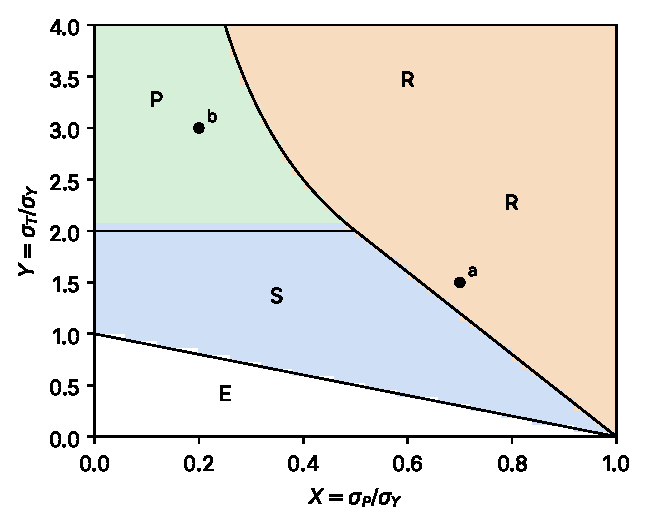
\includegraphics[width=0.5\textwidth]{figures/ch6/bree_diagram.pdf}
\caption{Bree diagram, perfect plasticity: elastic (E), elastic shakedown (S),
alternating plasticity (P) and ratchetting (R). Colours: regimes computed
cycle by cycle (30 cycles of 20 steps, 40 layers); lines: Bree's boundaries
$X+Y=1$, $Y=2$, $X+Y/4=1$, $XY=1$. Points (a) $X=0.7$, $Y=1.5$ and (b)
$X=0.2$, $Y=3$ are the cases of Sections~\ref{sec:cy-period}--\ref{sec:cy-dcm}.}
\label{fig:cy-bree-diagram}
\end{figure}

%======================================================================
\section{Two groups of equations on a time window}\label{sec:cy-split}
\index{global--local method}%
\subsection{Admissible and constitutive histories}
The quasi-static evolution problem of Chapter~\ref{ch:pl} (box in
Section~\ref{ssec:pl-bvp-eq}) splits into two groups of equations
(Figure~\ref{fig:pl-tonti}). Chapter~\ref{ch:pl-num} used the split at one
instant. Here it is used on a \emph{time window} $I$: one step $[t_n,t_\np]$,
the whole loading interval $[0,T]$, or one period. A \emph{history} on $I$ is
a set of fields $s=(\vu,\vz,\vSig)$ on $\Omega\times I$.
\begin{itemize}
  \item The \emph{admissible histories} $\Ad$ satisfy, at every instant of $I$,
  the kinematic conditions, equilibrium and the state laws
  $\sig=\bbC:(\eps[\vu]-\epsp)$, $\vq=-\bbD\valpha$, together with a
  \emph{closure} condition: the initial state $\vz(t_0)=\vz_0$, or the
  periodicity $\vz(t_0)=\vz(t_0+T)$. These equations are linear and global in
  space, and instantaneous in time: $\Ad$ is an affine set.
  \item The \emph{constitutive histories} $\Gcon$ satisfy the flow rule
  $\dot\vz\in N_{\Esig}(\vSig)$ at every point of $\Omega\times I$. These
  equations are nonlinear and local in space: each point carries its own
  evolution in time.
\end{itemize}
The solution is the history that belongs to both: $s\in\Ad\cap\Gcon$. Every
method of this chapter builds alternately a point of $\Ad$ (the \emph{global
stage}) and a point of $\Gcon$ (the \emph{local stage}).

\begin{proposition}[The two signs]\label{prop:cy-signs}
Let $s$, $s'$ be two histories on $I=[t_0,t]$ with the same closure data. If
$s,s'\in\Ad$, then
\[
  \int_{t_0}^{t}\!\!\int_\Omega(\vSig-\vSig')\cdot(\dot\vz-\dot\vz')\dd x\dd\tau
  =-\tfrac12\norm{(\vSig-\vSig')(t)}_E^2\le0
\]
when $\vSig(t_0)=\vSig'(t_0)$. If $s,s'\in\Gcon$, the same integral is
non-negative.
\end{proposition}
\begin{proof}
For admissible histories, the computation of the proof of
Theorem~\ref{thm:pl-unique} gives
$\displaystyle \frac{\dd}{\dd t}\tfrac12\norm{\Delta\vSig}_E^2=-\int_\Omega\Delta\vSig\cdot\Delta\dot\vz\dd x$,
because $\Delta\sig$ is self-equilibrated and $\Delta\dot\vu$ kinematically
admissible with zero data; integrate in time. For constitutive histories the
integrand is non-negative at every point by the monotonicity of the normal
cone (Corollary~\ref{cor:pl-monotone}).
\end{proof}
The uniqueness theorem of Chapter~\ref{ch:pl} is the case where $s$ and $s'$
are in both sets. The convergence proofs of
Section~\ref{sec:cy-latin} play the two signs against each other.

\subsection{The Melan decomposition}
\index{Melan decomposition}\index{residual stress!operator}%
The admissible set has an explicit structure. Let $(\vu^{el},\sig^{el})$ be the
\emph{fictitious elastic} response of the structure to the loads, the
response it would have without plasticity. For a plastic strain field $\epsp$
at zero load, let $\vw$ be the solution of the elastic problem with initial
strain $\epsp$:
\begin{equation}\label{eq:cy-eigen}
  \vw\in\Kad(\vzero,S_u),\qquad
  \int_\Omega\eps[\vw]:\bbC:\eps[\vv]\dd x=\int_\Omega\epsp:\bbC:\eps[\vv]\dd x
  \quad\forall\vv\in\Kad(\vzero,S_u),
\end{equation}
and define $\Pop\epsp=\eps[\vw]$ and $\Zop\epsp=\bbC:(\epsp-\Pop\epsp)$.
In finite elements, \eqref{eq:cy-eigen} is the system
$\mat{K}\mat{w}=\sum_e\int\mat{B}\T\mat{C}\,\epsp$ with the \emph{elastic}
stiffness, which is factorized once.

\begin{proposition}[Melan decomposition]\label{prop:cy-melan}
Every admissible history is of the form
\begin{equation}\label{eq:cy-melan}
  \eps=\eps^{el}+\Pop\epsp,\qquad
  \sig=\sig^{el}+\vrho,\qquad \vrho=-\Zop\epsp .
\end{equation}
The operator $\Pop$ is the projection onto the compatible strains, orthogonal
for the scalar product $\int_\Omega\vect a:\bbC:\vect b\dd x$. The residual
stress $\vrho$ is self-equilibrated; $\Zop$ is symmetric, positive
semi-definite, and its kernel is the set of compatible strains: a compatible
plastic strain produces no residual stress.
\end{proposition}
\begin{proof}
The problem is linear in the data $(\text{loads},\epsp)$; the elastic part
gives $\eps^{el}$, the plastic part gives $\Pop\epsp$ by~\eqref{eq:cy-eigen}.
By~\eqref{eq:cy-eigen}, $\vrho=\bbC:(\Pop\epsp-\epsp)$ satisfies
$\displaystyle \int_\Omega\vrho:\eps[\vv]\dd x=0$ for all admissible $\vv$; it is
self-equilibrated, and $\epsp-\Pop\epsp$ is orthogonal to the compatible strains.
If $\epsp=\eps[\vv]$ is compatible, $\Pop\epsp=\epsp$ and $\vrho=\vzero$.
\end{proof}
For the truss, $\Zop$ is the rank-one map~\eqref{eq:cy-truss-res}; for the
Bree vessel, $\Pop\varepsilon^p=\langle\varepsilon^p\rangle$ and
$\Zop\varepsilon^p=\tilde E(\varepsilon^p-\langle\varepsilon^p\rangle)$
by~\eqref{eq:cy-bree-melan}. In both cases the kernel of $\Zop$, the
compatible plastic strains, is the direction of ratchetting. Substituting the
decomposition~\eqref{eq:cy-melan} in the flow rule eliminates displacements
and equilibrium: the evolution problem becomes
\begin{equation}\label{eq:cy-reduced}
  \dot\vz\in N_{\Esig}\bigl(\sig^{el}(t)-\Zop\epsp,\ -\bbD\valpha\bigr),
  \qquad \text{closure on }\vz ,
\end{equation}
an evolution equation for the internal variables alone, local in time and
non-local in space through $\Zop$. It is a \emph{sweeping process} in the
sense of Moreau~\cite{Moreau1977}: the elastic domain, shifted by the elastic
stress $\sig^{el}(t)$, moves with the load and drags the internal variables.

\subsection{Three choices}
The methods of the chapter differ by three choices, which the rest of the
chapter takes one at a time.
\begin{gbox}{Window, closure, search directions}
\index{search directions}%
\begin{itemize}
  \item \textbf{Window} of one alternation of the local and global stages: one
  step (Chapter~\ref{ch:pl-num}), the interval $[0,T]$ (LATIN), one period
  (direct cyclic method), one streamline (stationary methods).
  \item \textbf{Closure}: initial state, periodicity $\vz(t_0)=\vz(t_0+T)$, or
  equality of the states upstream and downstream of a moving load.
  \item \textbf{Search directions}: the linear relations that link the point
  of $\Gcon$ to the previous point of $\Ad$ (local stage) and the next point of
  $\Ad$ to it (global stage): consistent tangent (Newton), elastic stiffness
  (initial strain), or a symmetric operator used in both stages (LATIN).
\end{itemize}
\end{gbox}

\begin{table}[h]
\centering\small
\renewcommand{\arraystretch}{1.15}
\begin{tabular}{@{}llll@{}}
\toprule
\sffamily method & \sffamily window & \sffamily closure & \sffamily global direction\\
\midrule
Newton (Box~5.3) & one step & initial & consistent tangent $\bbCalg$\\
initial strain (Box~6.1) & one step & initial & elastic $\bbC$\\
LATIN (Section~\ref{sec:cy-latin}) & $[0,T]$ & initial & symmetric $\mathbb L$, with relaxation\\
direct cyclic (Section~\ref{sec:cy-dcm}) & one period & periodic & elastic $\bbC$\\
stationary (Section~\ref{sec:cy-dcm}) & one streamline & upstream & elastic $\bbC$\\
\bottomrule
\end{tabular}
\caption{The methods of the chapter. In all of them the local stage is the
return map of Chapter~\ref{ch:pl-num} at fixed total strain, except LATIN,
whose local direction is $\mathbb L$.}
\label{tab:cy-methods}
\end{table}

\paragraph{A dictionary.}
The literature on these methods uses three notations. Ladev\`eze writes the
material in a ``normal formulation'' with internal variables $X$ and forces
$Y=AX$; Dang Van and Maitournam use internal parameters $a_k$ and forces
$A_k=Z:a_k$; Kondo and Maitournam~\cite{KondoMaitournam2023c} use the
irreversible forces $A=-\rho_0\,\partial\Psi/\partial(\cdot)$.
Table~\ref{tab:cy-dictionary} translates them into the notation of this book.
The only trap is a sign: Ladev\`eze's $Y$ and Dang Van--Maitournam's $A_k$ are
$-\vq$, while Kondo--Maitournam's force of a hardening variable is $\vq$.

\begin{table}[h]
\centering\small
\renewcommand{\arraystretch}{1.15}
\begin{tabular}{@{}llll@{}}
\toprule
 & \sffamily this book & \sffamily Ladev\`eze~\cite{LadevezeNCSM} & \sffamily Dang Van--Maitournam~\cite{DangVanMaitournam1993}\\
\midrule
Hooke, compliance & $\bbC$, $\bbS$ & $K$, $K^{-1}$ & $L$, $M$\\
hardening variables & $\valpha$ & $X$ & $a_k$\\
hardening law & $\vq=-\bbD\valpha$ & $Y=AX$ & $A_k=Z:a_k$\\
correspondence & & $X=\valpha$, $Y=-\vq$, $A=\bbD$ & $a_k=\valpha$, $A_k=-\vq$, $Z=\bbD$\\
dissipation & $\sig:\dot\eps^p+\vq\cdot\dot\valpha$ & $\sig:\dot\eps^p-Y\cdot\dot X$ & $\sig:\dot\eps^p-A_k\cdot\dot a_k$\\
flow rule & $\dot\vz\in\partial\varphi^\ast(\sig,\vq)$ & $(\dot\eps^p,-\dot X)=B(\sig,Y)$ & normality to $f(\sig,A_k)\le0$\\
admissible set & $\Ad$ & $A_d$ & KA, SA, state laws\\
constitutive set & $\Gcon$ & $\Gamma$ & integration along the path\\
\bottomrule
\end{tabular}
\caption{Notation of the LATIN method and of the direct methods in the
notation of this book (Table~\ref{tab:pl-dictionary}). In Kondo and
Maitournam~\cite[Sec.~2.6]{KondoMaitournam2023c}, with the plastic strain as
the kinematic variable, the force of $\epsp$ is $A_{\varepsilon^p}=\sig-\tbeta$
and the force of an isotropic variable is $q$.}
\label{tab:cy-dictionary}
\end{table}

%======================================================================
\section{Two orders for the same computations}\label{sec:cy-orders}
\index{direct method!order of the loops}\index{incremental method!order of the loops}%
\subsection{Step by step, or the whole history at once}
Discretize the window in instants $t_0<t_1<\dots<t_N$. Each method evaluates
the same two kinds of computations: a \emph{local} return map
$\vz_n=\mathcal R(\eps_n;\vz_{n-1})$ at each Gauss point and instant, and a
\emph{global} linear solve at each instant. They differ in the order of the
loops over the instants $n$ and over the iterations $k$
(Figure~\ref{fig:cy-orders}).

\providecommand{\cycorr}[2]{\draw[thick,#2,-{Latex[length=1.6mm]}] ($(#1)+(0.17,0.10)$)
   arc[start angle=-30,end angle=260,radius=0.2];}
\begin{figure}[h]
\centering
\begin{tikzpicture}[x=0.95cm,y=1cm,
  glob/.style={-{Latex[length=2mm]},thick,cphi},
  lab/.style={font=\small,align=left}]
  % (a) incremental
  \node[font=\sffamily\bfseries\small,right] at (-0.2,1.75) {(a) incremental};
  \draw[arr] (0,0) -- (9.6,0) node[right] {$t$};
  \foreach \x/\l in {0/t_0,3/t_{n-1},4.6/t_n,6.2/t_{n+1},9/t_N}
     {\draw (\x,0.1) -- (\x,-0.1) node[below] {$\l$};}
  \foreach \a/\b in {3/4.6,4.6/6.2}{
     \draw[glob,bend left=50] (\a,0.2) to (\b-0.05,0.35);
     \coordinate (c) at (\b,0.55); \cycorr{c}{cu}}
  \coordinate (c) at (3,0.55); \cycorr{c}{cu}
  \node[lab,cu] at (8.1,0.75) {$k=1,\dots,K_n$};
  % (b) direct
  \begin{scope}[yshift=-3.3cm]
  \node[font=\sffamily\bfseries\small,right] at (-0.2,2.25) {(b) whole history, iteration $k$};
  \draw[arr,gray] (0,0) -- (9.6,0) node[right,black] {$t$};
  \foreach \x in {0,1.25,2.5,3.75,5,6.25,7.5,8.75}{
     \draw[gray] (\x,0.08) -- (\x,-0.08);
     \draw[glob] (\x,1.55) -- (\x,1.05);
     \coordinate (c) at (\x,0.55); \cycorr{c}{cu}}
  \foreach \a/\b in {0/1.25,1.25/2.5,2.5/3.75,3.75/5,5/6.25,6.25/7.5,7.5/8.75}
     {\draw[cu,thick,-{Latex[length=1.6mm]}] (\a+0.22,0.67) to[bend left=35] (\b-0.2,0.67);}
  \draw[orange!80!black,thick,dashed,-{Latex[length=2mm]}] (8.75,-0.25) .. controls (8.6,-0.75) and (0.3,-0.75) .. (0,-0.25)
     node[pos=0.5,below,font=\scriptsize] {closure: $\vz(t_0)=\vz_0$, or $\vz(t_0)\gets\vz(t_N)$ (periodic)};
  \end{scope}
  % legend
  \begin{scope}[yshift=-5.0cm]
  \draw[glob] (0.1,0) -- (0.6,0); \node[lab,right] at (0.7,0) {global stage: equilibrium (elastic predictor)};
  \coordinate (c) at (0.35,-0.65); \cycorr{c}{cu}
  \node[lab,right] at (0.7,-0.6) {local stage: return map (plastic corrector), from $\vz(t_{n-1})$};
  \end{scope}
  % (c,d) lattice
  \begin{scope}[xshift=11.6cm,yshift=-0.4cm,x=0.5cm,y=0.42cm]
    \node[font=\sffamily\bfseries\small,right] at (-0.8,5.6) {(c) for $n$, for $k$};
    \foreach \i in {0,...,6}{\foreach \j in {0,...,3}{\fill[gray!60] (\i,\j) circle (1.4pt);}}
    \foreach \i in {0,...,5}{\draw[cu,thick,-{Latex[length=1.4mm]}] (\i,0.12) -- (\i,2.88);
       \draw[cphi,thick,-{Latex[length=1.4mm]}] (\i+0.08,3) .. controls (\i+0.5,3) and (\i+0.5,0) .. (\i+0.92,0);}
    \draw[cu,thick,-{Latex[length=1.4mm]}] (6,0.12) -- (6,2.88);
    \draw[->] (-0.5,-0.6) -- (6.6,-0.6) node[right,font=\scriptsize] {$n$};
    \draw[->] (-0.5,-0.6) -- (-0.5,3.6) node[above,font=\scriptsize] {$k$};
  \end{scope}
  \begin{scope}[xshift=11.6cm,yshift=-3.7cm,x=0.5cm,y=0.42cm]
    \node[font=\sffamily\bfseries\small,right] at (-0.8,5.6) {(d) for $k$, for $n$};
    \foreach \i in {0,...,6}{\foreach \j in {0,...,3}{\fill[gray!60] (\i,\j) circle (1.4pt);}}
    \foreach \j in {0,...,3}{\draw[cu,thick,-{Latex[length=1.4mm]}] (0.12,\j) -- (5.88,\j);}
    \foreach \j in {0,...,2}{\draw[cphi,thick,-{Latex[length=1.4mm]}] (5.95,\j+0.1) .. controls (3,\j+0.6) and (3,\j+0.4) .. (0.05,\j+0.9);}
    \draw[->] (-0.5,-0.6) -- (6.6,-0.6) node[right,font=\scriptsize] {$n$};
    \draw[->] (-0.5,-0.6) -- (-0.5,3.6) node[above,font=\scriptsize] {$k$};
  \end{scope}
\end{tikzpicture}
\caption{Two orders for the same computations. (a) Incremental: the elastic
predictor of the increment $t_{n-1}\to t_n$ (green) and the plastic corrector
(blue) are repeated at fixed $t_n$ until equilibrium; then the next step
starts. (b) Whole history: at iteration $k$ the global stage solves the
elastic problems of all the instants at once (they are independent), then
the local stage sweeps the history at each Gauss point, and the closure
condition starts the next iteration. (c), (d) The lattice of the computations
$(t_n,k)$, visited column by column or row by row.}
\label{fig:cy-orders}
\end{figure}

The incremental method of Chapter~\ref{ch:pl-num} loops \emph{for $n$, for
$k$}: it converges the equilibrium of $t_n$ before it looks at $t_\np$. The
iteration on the whole history loops \emph{for $k$, for $n$}: it visits all
the instants with the same (wrong) data, and corrects them all at the next
iteration. With the elastic stiffness in the global stage, the two
algorithms are written below; Box~6.1 is the modified
Newton method of Box~5.3.

\begin{gbox}{Box 6.1\quad Initial-strain iteration, step by step}
\index{initial-strain method}%
\begin{enumerate}[label=\textbf{\arabic*.},leftmargin=1.6em]
  \item \textbf{Step.} For $n=1,\dots,N$, start from $\mat{u}^{(0)}=\mat{u}_{n-1}$.
  \item \textbf{Local stage.} At each Gauss point,
  $(\sig^{(k)},\vz^{(k)})=\mathcal R(\mat{B}\mat{u}^{(k)};\vz_{n-1})$.
  \item \textbf{Global stage.} Solve
  $\mat{K}\,\delta\mat{u}=\mat{F}^{\mathrm{ext}}_n-\sum_e\int\mat{B}\T\sig^{(k)}$
  with the elastic stiffness $\mat{K}$, factorized once;
  $\mat{u}^{(k+1)}=\mat{u}^{(k)}+\delta\mat{u}$.
  \item \textbf{Test.} Repeat 2--3 until the residual is small; store
  $\vz_n=\vz^{(k)}$ and go to the next step.
\end{enumerate}
\end{gbox}

\begin{gbox}{Box 6.2\quad Iteration on the whole history}
\index{direct cyclic method!Box 6.2}%
\begin{enumerate}[label=\textbf{\arabic*.},leftmargin=1.6em]
  \item \textbf{Initialization.} $\epsp(t_n)=\vzero$ for all $n$ (or a guess);
  closure state $\vz(t_0)$.
  \item \textbf{Global stage.} For every instant $t_n$, solve the elastic problem
  with initial strain: $\mat{K}\mat{u}_n=\mat{F}^{\mathrm{ext}}_n+\sum_e\int\mat{B}\T\mat{C}\,\epsp(t_n)$
  (one factorization, $N$ independent solutions); $\eps_n=\mat{B}\mat{u}_n$.
  \item \textbf{Local stage.} At each Gauss point, sweep the history:
  $\vz(t_n)=\mathcal R(\eps_n;\vz(t_{n-1}))$, $n=1,\dots,N$.
  \item \textbf{Closure.} Initial condition: $\vz(t_0)=\vz_0$. Periodic
  (direct cyclic method): $\vz(t_0)\gets\vz(t_N)$.
  \item \textbf{Test.} Repeat 2--4 until the stresses of the two stages agree
  at all instants (and, if periodic, $\vz(t_N)=\vz(t_0)$).
\end{enumerate}
\end{gbox}

\subsection{What each order guarantees}
\paragraph{Why time stepping is the standard.}
The evolution problem~\eqref{eq:cy-reduced} with an initial condition is a
Cauchy problem, and it is causal: the state at $t$ depends on the past only.
The implicit Euler scheme for a sweeping process, Moreau's \emph{catching-up
algorithm}~\cite{Moreau1977}, is the return map; it is at the same time the
proof of existence of the solution and the algorithm that computes it. Each
step is the minimization of a strictly convex incremental potential
(Theorem~\ref{thm:pn-W}), with a unique solution and a globally convergent
Newton method; the next step starts from a converged state, close to the
solution; and the return map is contractive
(Theorem~\ref{thm:pn-contract}), so that an error made in a step is not
amplified by the following ones. Consistency and stability give the
convergence of the time discretization. Everything is local in time, and so
are the guarantees.

\paragraph{What the whole-history iteration risks.}
\index{ratchetting!non-convergence of direct methods}%
The iteration of Box~6.2 is a fixed-point iteration on
histories, $\epsp\gets\mathcal R_{[t_0,t_N]}(\eps^{el}+\Pop\epsp)$, and the
properties of each step do not transfer to it.
\begin{itemize}
  \item No theorem covers the pair ``return map at fixed total strain, elastic
  stiffness'' on a window. The LATIN theorem of Section~\ref{sec:cy-latin}
  needs other directions and a relaxation.
  \item Rate-independent plasticity has no fading memory. The return map is
  only non-expansive with respect to $\vz_{n-1}$, so that an error made at
  $t_n$ is carried unchanged to all later instants by the local sweep.
  Figure~\ref{fig:cy-truss-lattice}b shows it: a correction made at the first
  plastic instant reappears at every later instant, iteration after
  iteration, while the incremental method confines its iterations to the
  plastic steps.
  \item With the periodic closure, an error that is constant in time is not
  damped by the time coupling at all. In plasticity this is the kernel of
  $\Zop$: a compatible plastic strain added to a periodic state gives another
  periodic state. The iteration may converge to a periodic state that depends
  on its starting point, or not converge at all if the structure ratchets
  (Sections~\ref{sec:cy-period}--\ref{sec:cy-dcm}).
  \item The iterates are not states of any loading history; there is no energy
  that decreases from one iteration to the next unless the directions are
  chosen for it, as in LATIN.
\end{itemize}

\begin{figure}[h]
\centering
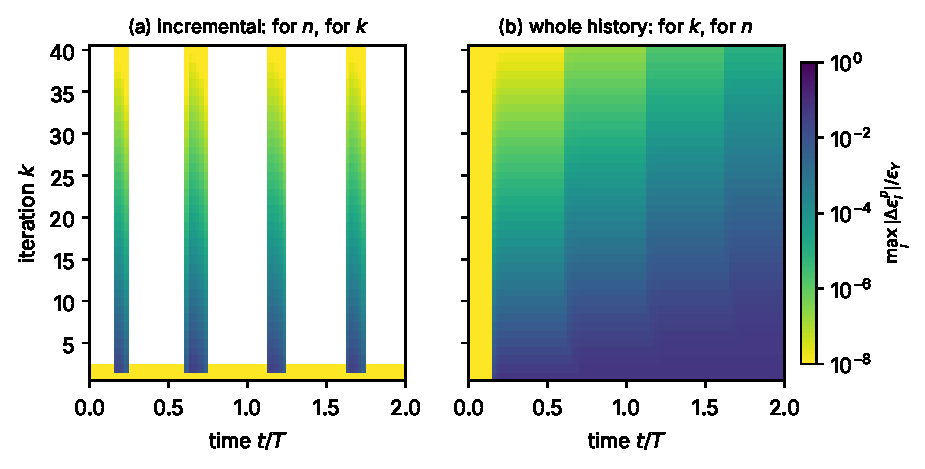
\includegraphics[width=0.85\textwidth]{figures/ch6/truss_lattice.pdf}
\caption{The lattice of Figure~\ref{fig:cy-orders} computed for the truss
($H=0.05E$, $Q_2=N_0$, $Q_1=1.2N_0\sin t$, two periods of 40 steps): size of the
plastic correction $\max_i|\Delta\varepsilon^p_i|$ at each instant $t_n$ and
iteration $k$. (a) Incremental initial-strain iteration (Box~6.1):
2 iterations at the elastic steps, up to 46 at the plastic ones, 982 local
evaluations in all. (b) Iteration on the whole history
(Box~6.2, initial condition): the corrections made at the
first plastic instants are carried to the end of the window; 40 iterations
($3200$ local evaluations) reach an indicator of $3\times10^{-6}$.}
\label{fig:cy-truss-lattice}
\end{figure}

\paragraph{When it pays.}
The whole-history iteration wins when its strengths matter more than its
risks:
\begin{itemize}
  \item \emph{Confined plasticity.} By~\eqref{eq:cy-melan}, the elastic
  prediction is exact outside the plastic zone, and the correction couples
  the plastic points only through $\Zop$ restricted to the plastic zone. A
  small plastic zone in an elastic structure (contact, notches, the skin of a
  thermal shock) gives a fast contraction.
  \item \emph{One loop instead of two.} Cycle after cycle, the incremental
  method converges the equilibrium of every step of every transient cycle,
  which is then thrown away. The direct cyclic method converges the
  equilibrium and the periodicity together.
  \item \emph{Cheap iterations.} The global stage uses the elastic stiffness,
  factorized once; the instants are independent and can be compressed in a
  Fourier or wavelet basis in time~\cite{MaitournamPommierThomas2002}; the
  local stage is parallel in space.
\end{itemize}
Figure~\ref{fig:cy-truss-process} compares the costs on the truss. For three
bars, factorizing the tangent is free, and the cycle-by-cycle computation
needs fewer local evaluations than the direct cyclic method (3750 against
13\,200 to reach $10^{-6}\varepsilon_Y$); Anderson acceleration of the period
map (Section~\ref{sec:cy-period}) needs four cycles. In a finite element model
the balance changes: the incremental method refactorizes the tangent at
every Newton iteration, the direct cyclic method never does, and Maouche et
al.~\cite{MaoucheMaitournamDangVan1997} report a computation of fretting
contact ten times faster in gross slip (3\,h against 30\,h for 74 cycles) and
twice as fast in partial slip.

\begin{figure}[h]
\centering
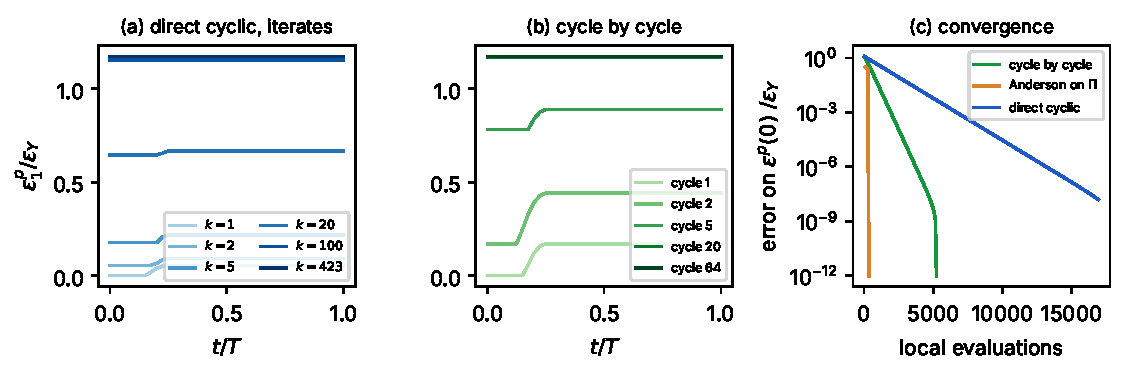
\includegraphics[width=\textwidth]{figures/ch6/truss_process.pdf}
\caption{Truss, $H=0.05E$, $Q_2=N_0$, $Q_1=1.2N_0\sin t$, one period of 40 steps.
(a) Plastic strain of bar~1 over the period, iterates $k$ of the direct cyclic
method (Box~6.2, periodic closure). (b) The same quantity in
cycles 1 to 64 of the incremental computation. (c) Error on the periodic
state against the number of local evaluations: cycle by cycle (Newton,
Box~5.3), Anderson acceleration of the period map, direct cyclic method.}
\label{fig:cy-truss-process}
\end{figure}

%======================================================================
\section{Search directions and the LATIN method}\label{sec:cy-latin}
\index{LATIN method}\index{large time increment method|see{LATIN method}}%
\draftnote{To be written. Content: Ladev\`eze's two-direction framework for one
step (Ch.~3 of~\cite{LadevezeNCSM}): local direction ``vertical'' (total strain
fixed) = return map; global direction tangent (Newton) or elastic (initial
strain, Nguyen 1977); convergence factor $E/(E+C)$ of the filament. LATIN on
$[0,T]$: directions on the rates, local stage with $\mathbb L$, global stage
Maxwell-type marched in time; theorem 4.1 of~\cite{LadevezeNCSM} with the
relaxation $\mu>0$, partial convergence for $\mu=0$ in statics (Thm.~4.3);
computation on the truss: with $\mu=0$ the indicator stalls although the
constitutive iterate is exact, with $\mu=0.3$ it converges (cy\_core.latin).
Radial (PGD) approximation and wavelets (Comte et al.) in one paragraph.}

%======================================================================
\section{Cyclic loads: the period map}\label{sec:cy-period}
\index{period map}\index{shakedown!period map}%
\draftnote{To be written. Content: adaptation, accommodation, rochet (Maitournam
Ch.~4); Halphen's results; contraction of distances (Proposition~\ref{prop:cy-signs});
period map non-expansive for the seminorm $\int\epsp:\Zop\epsp+\valpha\cdot\bbD\valpha$;
Picard, Krasnoselskii--Mann, Anderson; Bree case (a) with $H=0.02E$: 261 cycles,
Anderson 13; non-uniqueness: case (b), two exact periodic states differing by a
constant residual stress of $0.3\sigma_0$ (figure bree\_nonunique); local shakedown
theorem for linear kinematic hardening (Maitournam Sec.~4.4.3).}

%======================================================================
\section{The direct cyclic and stationary methods}\label{sec:cy-dcm}
\index{direct cyclic method}\index{stationary method}%
\draftnote{To be written. Content: Box~6.2 with periodic closure
(Akel--Nguyen; Maouche et al.\ 1997); Fourier in time (Maitournam, Pommier,
Thomas 2002); figures bree\_process (iterates in space at $T/2$) and
bree\_ratchet (drift of $\langle\varepsilon^p\rangle$, $0.060\varepsilon_Y$ per
iteration, residual stress converged to $10^{-15}$). Stationary methods
(Dang Van--Maitournam 1993): moving frame, PPSM, DSM, uniqueness; Cast3M
procedure @STATIO.}

%======================================================================
\section{Zarka's simplified analysis}\label{sec:cy-zarka}
\index{Zarka's method}%
\draftnote{To be written. Content: transformed parameter $Y=H\epsp-\vrho$; local
criterion centred on $\sig^{el}(t)$; elastic shakedown iff the intervals
(balls) intersect (Mandel--Halphen--Zarka 1977); projection of the state after
the first half-cycle; linear problem $(H\,\mathbb I+\Zop)\epsp=Y$; exact on the
truss and on Bree case S (cy\_core.zarka); Amiable et al.\ 2006; Cast3M @ZACPLUS.}

%======================================================================
\section{A map of the direct methods}\label{sec:cy-map}
\draftnote{To be written: one table (linear matching, residual stress
decomposition, optimal control of Peigney--Stolz, cycle jump, multi-time-scale
LATIN, PGD, Brezis--Ekeland--Nayroles), each with one line and one reference.}

%======================================================================
\framepart{Summary}
\begin{gbox*}
\begin{itemize}
  \item \textbf{Two model problems}: the three-bar truss (one redundancy,
  self-stresses $\gamma(1,1,-\sqrt2)$, limit load $(1+\sqrt2)N_0$) and the Bree
  vessel (residual stress $-\tilde E(\varepsilon^p-\langle\varepsilon^p\rangle)$,
  Bree diagram). Both show elastic shakedown, alternating plasticity and
  ratchetting.
  \item \textbf{Two groups of equations}: admissible histories $\Ad$ (linear,
  global, with a closure condition) and constitutive histories $\Gcon$
  (nonlinear, local); the solution is $\Ad\cap\Gcon$. On $\Ad$ the dissipation
  of a difference is non-positive, on $\Gcon$ non-negative.
  \item \textbf{Melan}: $\eps=\eps^{el}+\Pop\epsp$, $\sig=\sig^{el}-\Zop\epsp$;
  compatible plastic strains, the kernel of $\Zop$, give no residual stress and
  are the direction of ratchetting.
  \item \textbf{Two orders}: incremental (for $n$, for $k$) inherits the
  guarantees of each step; the iteration on the whole history (for $k$, for
  $n$) has none in general, carries errors forward without damping, and with a
  periodic closure may converge to non-unique states or drift. It pays when
  plasticity is confined, when many transient cycles are avoided, and when
  factorizations are expensive.
\end{itemize}
\draftnote{Summary of Sections 6.4--6.8 to be added.}
\end{gbox*}

\framepart{Exercises}\label{sec:cy-exo}
The computational exercises use the module \texttt{cy\_core}, which contains the
two model problems, the return map with a search direction, the global stage,
the incremental and whole-history solvers, the period map and Zarka's
estimate.\draftnote{Problems with code to be added with Sections 6.4--6.8.}

\framesub{Short questions}

\exercise{Regimes of the three-bar truss}\label{exo:cy-q-truss}
\index{three-bar truss!exercise}%
Elastic--perfectly plastic bars, $N_0=S\sY$. Using~\eqref{eq:cy-truss-el} and
Melan's theorem, find the regime under (a) $Q_1=1.1N_0(1-\cos t)$, $Q_2=0$;
(b) $Q_1=1.9N_0\sin t$, $Q_2=0$. (c) Under $Q_2=N_0$ and $Q_1=1.2N_0\sin t$,
show that the plastic elongation $(a,-a,0)$ is compatible, and explain why it
can grow without bound.
\begin{solution}
(a) $N^{el}_3=2Q_1/(2+\sqrt2)$ varies in $[0,\,1.289N_0]$ and $N^{el}_{1,2}$ in
$[0,\,0.644N_0]$. The constant residual field $\gamma(1,1,-\sqrt2)$ with
$\gamma=0.25N_0$ gives $N_3\in[-0.354,\,0.935]N_0$ and
$N_{1,2}\in[0.25,\,0.894]N_0$, inside $[-N_0,N_0]$: elastic shakedown (Melan).
Bar~3 yields in the first cycle since $\max N^{el}_3>N_0$. (b) The range of
$N^{el}_3$ is $4\times1.9/(2+\sqrt2)\,N_0=2.23N_0>2N_0$; no residual field can
bring it into $[-N_0,N_0]$: bar~3 yields in every cycle, alternating
plasticity. (c) $\delta^p_1+\delta^p_2-\sqrt2\,\delta^p_3=0$, so
by~\eqref{eq:cy-truss-res} the residual forces vanish: the increment is the
elongation of a vertical displacement of $O$. Nothing in the stresses
resists it; the computation gives $a=0.4\,\delta_Y$ per cycle.
\end{solution}

\exercise{Melan decomposition of the Bree vessel}\label{exo:cy-q-bree}
\index{Bree problem!exercise}%
From~\eqref{eq:cy-bree}, derive~\eqref{eq:cy-bree-melan}. Show that
$\Pop\varepsilon^p=\langle\varepsilon^p\rangle$ and that the kernel of $\Zop$ is
the set of uniform plastic strains. What does a uniform plastic strain mean
for the vessel?
\begin{solution}
Take the mean of~\eqref{eq:cy-bree} through the wall: $\langle x\rangle=0$, so
$\sigma_P=\tilde E(\varepsilon-\langle\varepsilon^p\rangle)$ and
$\varepsilon=\sigma_P/\tilde E+\langle\varepsilon^p\rangle$; substituting,
$\sigma=\sigma^{el}-\tilde E(\varepsilon^p-\langle\varepsilon^p\rangle)$. The
compatible strains are the uniform ones ($\mat{B}$ is a column of ones), and
$\Pop$ is the orthogonal projection on them, the mean. $\Zop\varepsilon^p=0$
if and only if $\varepsilon^p$ equals its mean. A uniform hoop plastic strain
is a permanent increase of the radius: the vessel swells without stress. It
is the ratchet strain of the Bree problem.
\end{solution}

\begin{chapterbib}{99}
\bibitem{Bree1967} J.~Bree, Elastic-plastic behaviour of thin tubes subjected to internal pressure and intermittent high-heat fluxes with application to fast-nuclear-reactor fuel elements, \emph{J. Strain Anal.} 2 (1967) 226--238.
\bibitem{DangVanMaitournam1993} K.~Dang Van, M.~H.~Maitournam, Steady-state flow in classical elastoplasticity: applications to repeated rolling and sliding contact, \emph{J. Mech. Phys. Solids} 41 (1993) 1691--1710.
\bibitem{KondoMaitournam2023c} D.~Kondo, H.~Maitournam, Thermodynamics of irreversible processes: formulation of constitutive models, Chapter~2 in J.~Besson et al., \emph{MEALOR II: Damage Mechanics and Local Approach to Fracture}, 2023, 5--38.
\bibitem{LadevezeNCSM} P.~Ladev\`eze, \emph{Nonlinear Computational Structural Mechanics: New Approaches and Non-Incremental Methods of Calculation}, Springer, 1999.
\bibitem{Maitournam2012c} H.~Maitournam, \emph{M\'ecanique des structures an\'elastiques: comportement, chargements cycliques et fatigue}, course notes MEC562, \'Ecole polytechnique, 2012.
\bibitem{MaitournamPommierThomas2002} M.~H.~Maitournam, B.~Pommier, J.-J.~Thomas, D\'etermination de la r\'eponse asymptotique d'une structure an\'elastique sous chargement thermom\'ecanique cyclique, \emph{C. R. M\'ecanique} 330 (2002) 703--708.
\bibitem{MaoucheMaitournamDangVan1997} N.~Maouche, M.~H.~Maitournam, K.~Dang Van, On a new method of evaluation of the inelastic state due to moving contacts, \emph{Wear} 203--204 (1997) 139--147.
\bibitem{Moreau1977} J.-J.~Moreau, Evolution problem associated with a moving convex set in a Hilbert space, \emph{J. Differential Equations} 26 (1977) 347--374.
\end{chapterbib}
